\thispagestyle{empty}
\begin{center}
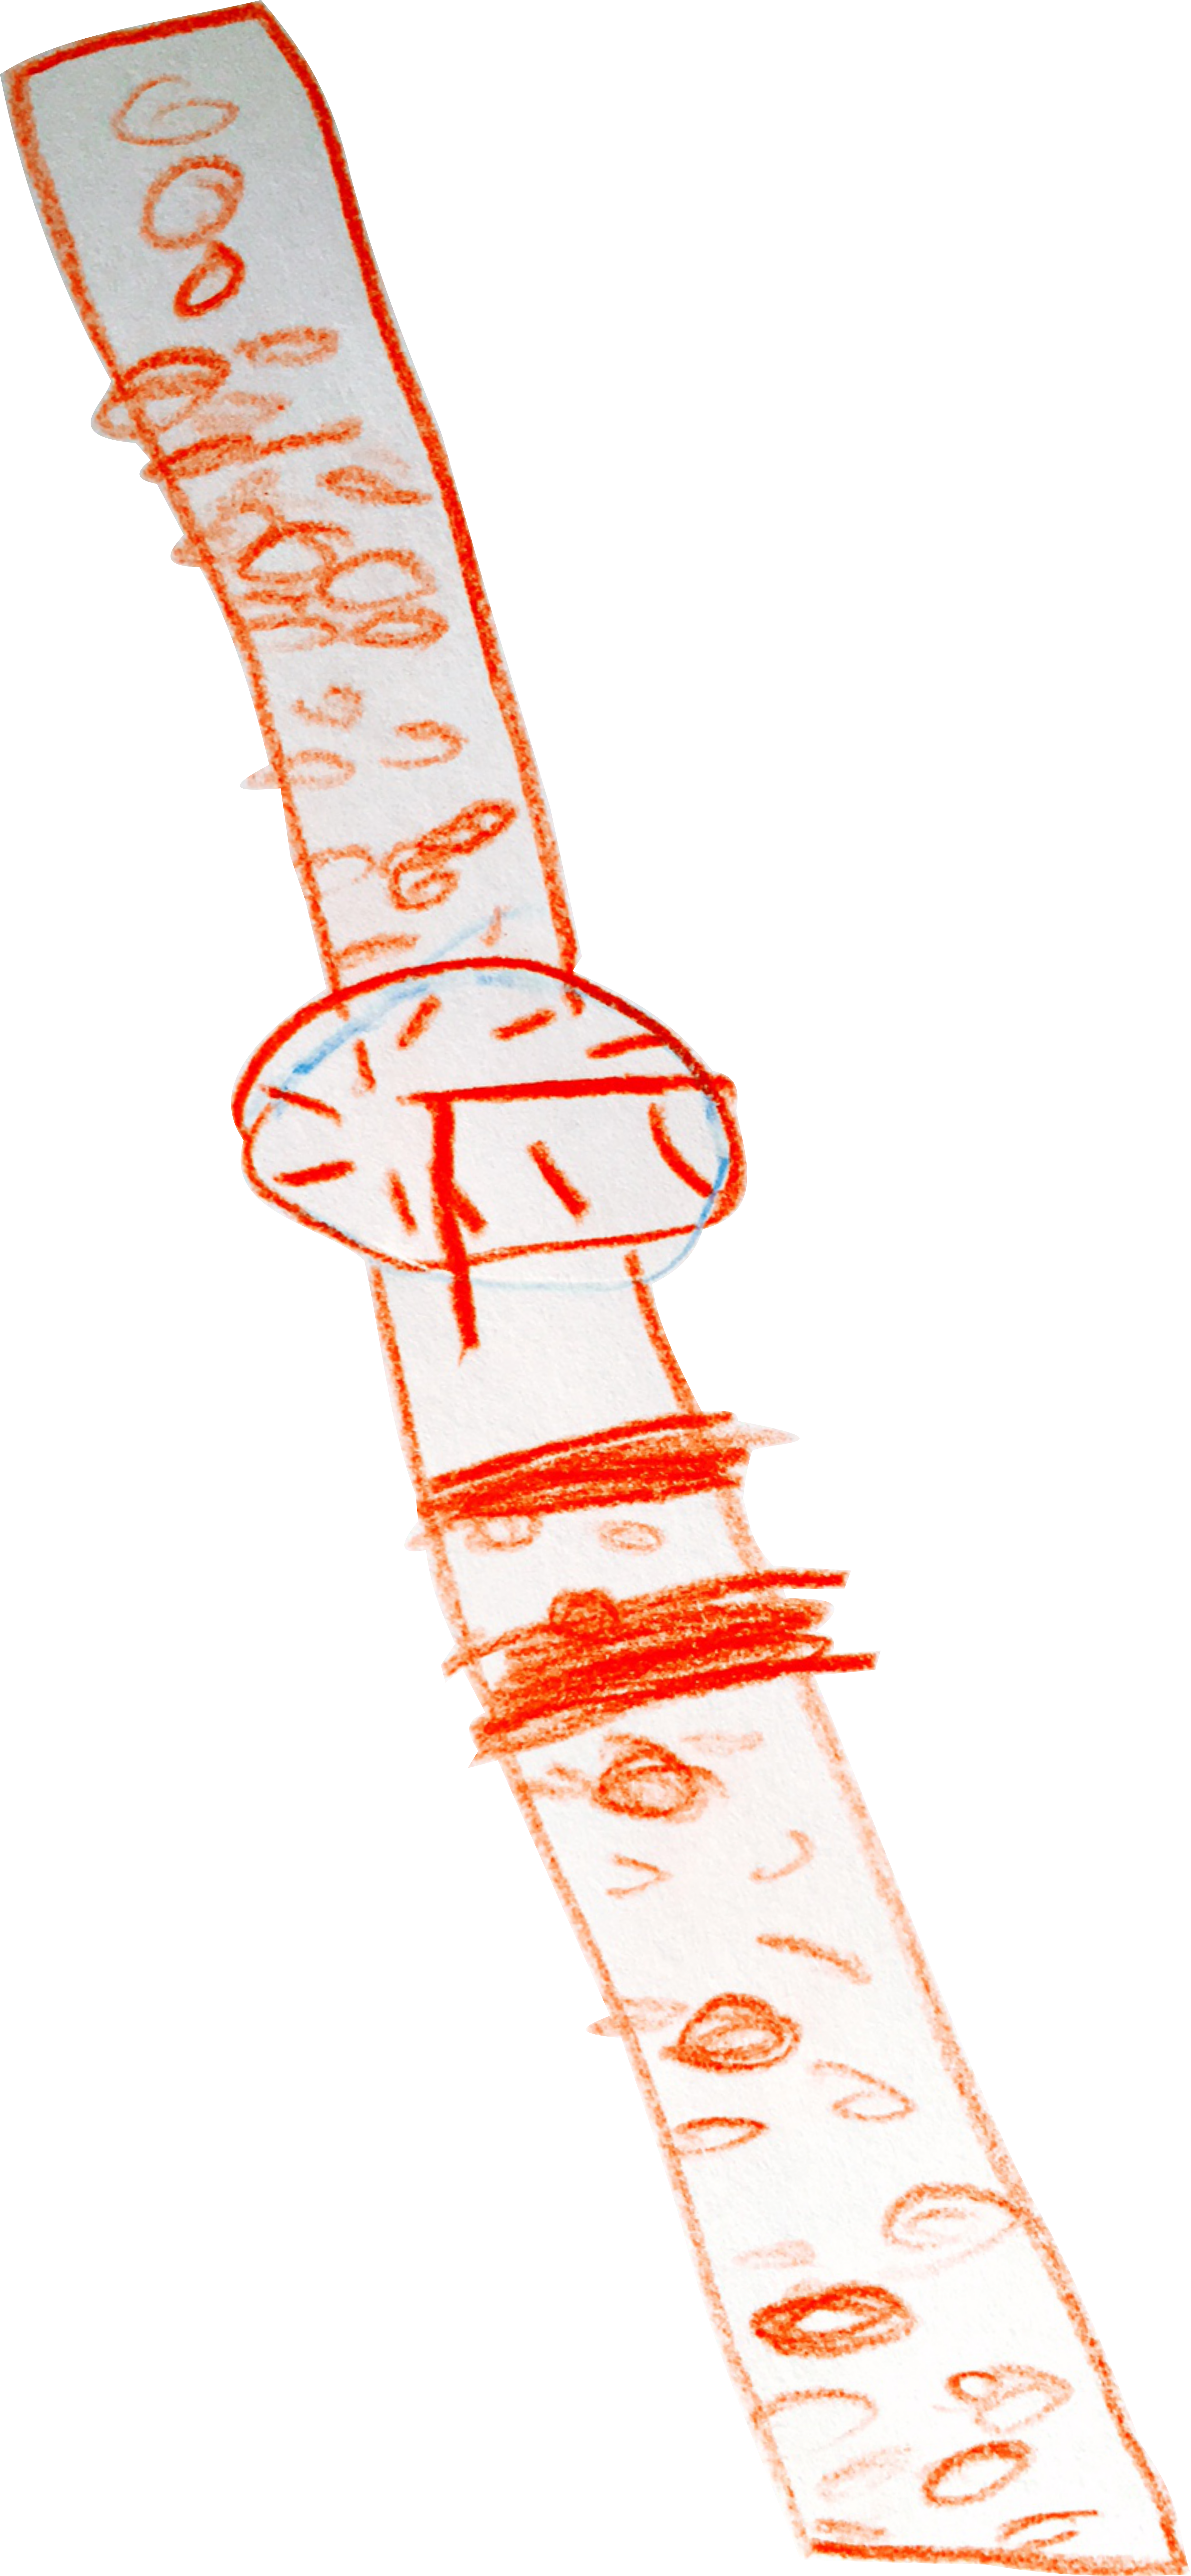
\includegraphics[height=.8\textheight]{./bilder/160120_uhr.png}
\end{center}
\vskip 2cm
{\Huge\color{farbe}\hfill{\tt{¨Uber den Staub}}}
\addcontentsline{toc}{chapter}{}
\newpage
%%%%%%%%%%%%%%%%%%%%%%%%%%%%%%%%%%%%%%%%%%%%%%%%%%%%%%%%%%%%%%%%%%%%%%%%%%%%%%%
\lettrine[lines=2, lhang=.2, loversize=.25, lraise=0.05, findent=0.1em,
nindent=0em]{W}{}aterieforscher unterscheiden verschiedene Schadklassen von Materialien. Staub gehört zur höchten Klasse, den ganzschädlichen Materialien. Eine Klasse darunter befindet sich beispielsweise Plutonium, dass zur Klasse der zweckschädlichen Materialien gehört. Die Schadklasse von Staub ist für den Wissenschaftler damit eine Höhere als Plutonium.  

Erlauben Sie mir bitte, dies als Anlass zu verstehen, der öffentlichkeit dieses Material etwas Näher zu bringen. 

Staub entsteht ganz allgemein an der Staubquelle als Nucleii. Bekannte Staubquellen sind beispielsweise Hypotrichose und andere Ursachen von Haarausfall. 


\vfill
